%Dokumentinnstillinger:---------------------------------
%Ved å google flitting kan du finne ut hva de forskjellige tingene her betyr, og hvordan du kan gjøre eventuelle endringer.
\documentclass[a4paper,11pt,norsk]{article}
\usepackage[utf8]{inputenc}
\usepackage{a4wide}
\usepackage{lmodern}
\usepackage[T1]{fontenc}
\usepackage{babel}
\setlength{\parindent}{0pt} 
\setlength{\parskip}{2ex}
\usepackage{fixltx2e}
\usepackage{amsmath}
\usepackage[pdftex, pdfborderstyle={/S/U/W 0}]{hyperref}
\usepackage{graphicx}
\usepackage[font=small,labelfont=bf]{caption}
\usepackage{tabularx}
\usepackage{multirow}
\usepackage{float}
\usepackage[RPvoltages]{circuitikz}




\begin{document}

%Headingdel:---------------------------------------------
\begin{minipage}[c]{0.15\textwidth}

\includegraphics[width=2.0cm]{D1/Images/elsys_pos_staaende_ntnu.png}  
\end{minipage}
\begin{minipage}[c]{0.85\textwidth}

\renewcommand{\arraystretch}{1.7}
\large 
\begin{tabularx}{\textwidth}{|X|X|}
\hline
\multicolumn{2}{|l|}{} \\
\multicolumn{2}{|l|}{\huge \textbf{Designnotat}} \\
\multicolumn{2}{|l|}{}  \\
\hline
\multicolumn{2}{|l|}{Tittel: 
%Skriv inn tittel her:------------------------------------------
Frekvensmultiplikator
} \\
\hline
\multicolumn{2}{|l|}{Forfatter: 
%Skriv inn forfattere her:--------------------------------------
Freider Engstrøm Fløan
} \\
\hline
%Skriv inn versjon og dato her her:-----------------------------
Versjon: 2.0 & Dato: 06.05.22
\\
\hline 
\end{tabularx}
\end{minipage}
\normalsize

%Automatisk generert innholdsfortegnelse:------------------

\setlength{\parskip}{0ex}
\renewcommand{\baselinestretch}{0.1}\normalsize
\tableofcontents
\renewcommand{\baselinestretch}{1.00}\normalsize
\setlength{\parskip}{2ex}
\rule{\textwidth}{1pt}
\label{sec:innledning}

\newpage



%Selve rapporten:------------------------------------------
\section{Problembeskrivelse}
\label{sec:problembeskrivelse}

Vi vil ta for oss design av et system, vist i figur \ref{fig:1}, som skal gi ut et multiple av inngangssignalet. Systemet tar inn et signal $x_1(t)$ = $A_1cos(\omega t)$, og gir ut et signal $x_k(t)$ = $A_kcos(\omega k t + \phi)$,  $k \in \mathbb{N}$.  
Endringer i faseforskyving og amplitude på utgangssignalet er ikke relevant for resultatet. Testet systemet skal designes slik at utgangssignalet har dobbelt frekvens fra inngangssignalet.

Utgangssignalet $x_k(t)$ skal analyseres ved hjelp av SDR (Signal-to-Distortion-Ration)
for å kunne si noe om kvaliteten på systemet, der stor SDR-verdi indikerer et godt resultat. 

\begin{figure}[H]
  \centering
  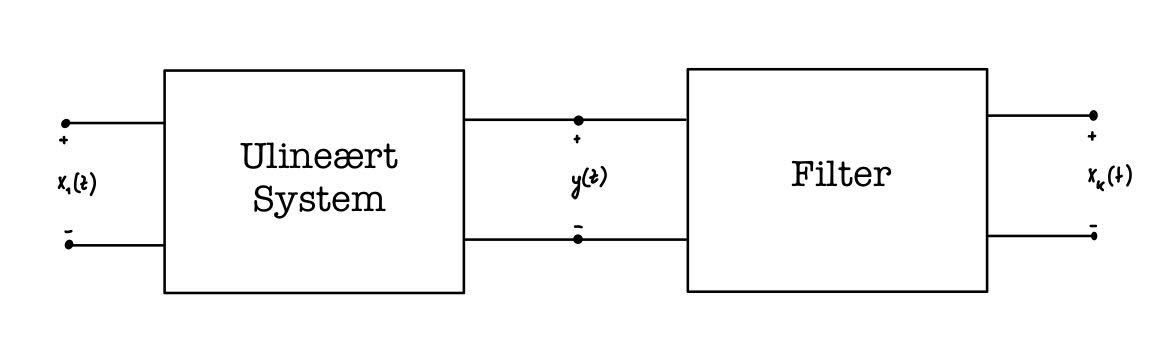
\includegraphics[scale=0.7]{D1/Images/system.jpg}
  \caption{Et frekvensmultiplikator-system.}
  \label{fig:1}
\end{figure}

\section{Prinsipiell løsning}
\label{sec:prinsipielllosning}


Ved å utnytte egenskapene til linære og ikke-lineære kretskomponenter kan frekvenser både blokkeres og forbli uendret ut ifra hvordan de er koblet sammen som deler systemet inn i to delsystemer. Som vist i figur \ref{fig:1} sendes signalet først gjennom et ikke-lineært delsystem, der sinussignalet blir forvrengt, deretter gjennom et filter som slipper gjennom ønsket frekvens. 

\subsection{Halvbølge likeretter}
\label{sub:ulineeartsystem}
Et sinussignal som sendes gjennom et lineært system vil alltid ha samme frekvens ved utgangen. Derfor er det nødvendig med et ulineært system for å kunne forvrenge inngangssignalet som genererer overharmoniske frekvenser. En måte å løse dette på kan være ved hjelp av en ulineær kretskomponent som en diode. I figur \ref{fig:2} er det koblet en diode i serie med en resistor, der utgangssignalet $y(t)$, vist i figur \ref{fig:3}, er målt over resistoren, også kjent som en halvbølge likeretter. 

\begin{figure}[H]
    \centering
    \begin{minipage}{0.45\textwidth}
        \centering
        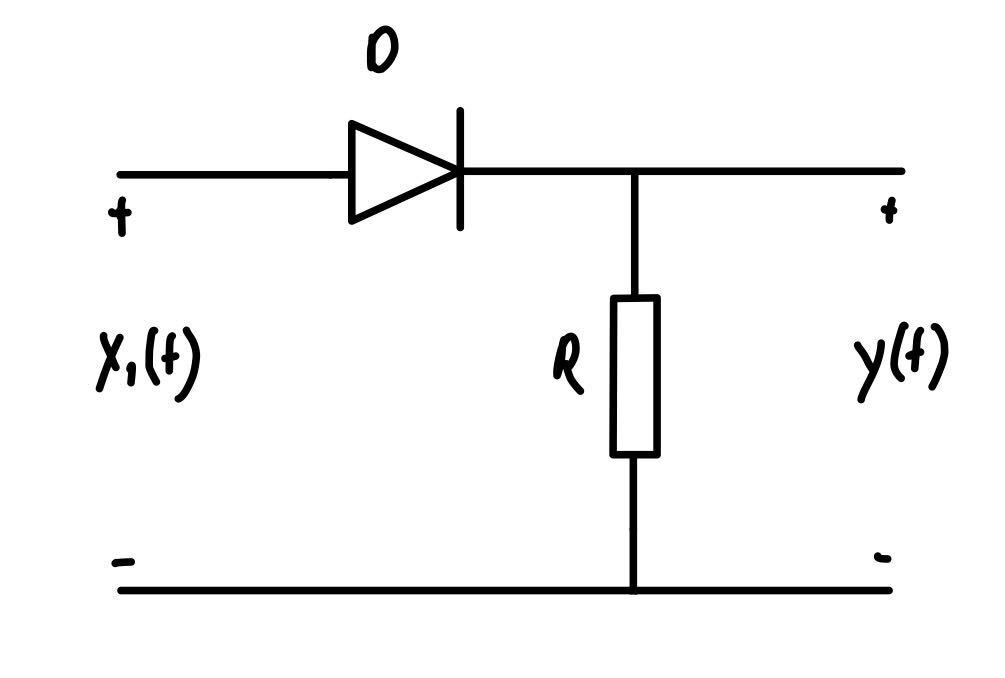
\includegraphics[width=0.8\textwidth]{D1/Images/dioderesistor.jpg}  \caption{Halvbølge likeretter med en diode og en resistor}
        \label{fig:2}
    \end{minipage}\hfill
    \begin{minipage}{0.45\textwidth}
        \centering
        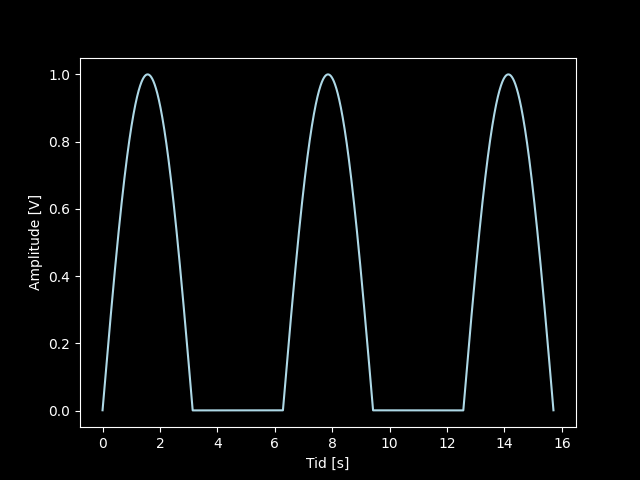
\includegraphics[width=1\textwidth]{D1/Images/halfwave.png} 
        \caption{Osiloskopanalyse av utgangssignalet $y(t)$}
        \label{fig:3}
    \end{minipage}
\end{figure}

Utgangssignalet $y(t)$ vist i figur \ref{fig:3} kan, ved hjelp av en spektrumsanalysator, beskrives som en sum av flere sinussignaler med forskjellige frekvenser. Disse er overharmoniske frekvenser fra signalet $y(t)$ og kan beskrives matematisk ved hjelp av fourier serier:

\begin{equation*}
    x_1(t) =  y(t + n T),  n \in \mathbb{Z},
\end{equation*}

\begin{equation*}
    x_1(t) =  \frac{a_0}{2} + \displaystyle\sum_{n=1}^{\infty} a_n cos(2\pi \frac{n }{T}t) + \displaystyle\sum_{n=1}^{\infty} b_n sin(2\pi \frac{n}{T}t),
\end{equation*}

der $a_0$ og $b_0$ er fourier koeffisientene som kan regnes ut ved:

\begin{equation}
    a_0 = \frac{2}{T} \int_{0}^{T} x(t)cos(2\pi \frac{n}{T}t) \,dx ,
    \label{eq:a0}
\end{equation}
\begin{equation}
    b_0 = \frac{2}{T} \int_{0}^{T} x(t)sin(2\pi \frac{n}{T}t) \,dx ,
    \label{eq:b0}
\end{equation}

I likningene (\ref{eq:a0}) og (\ref{eq:b0}) er frekvensene til cosinus og sinus gitt ved $\frac{1}{T}$, $\frac{2}{T}$, $\frac{3}{T}$... altså er de multipler av grunnfrekvensen $\frac{1}{T}$. Dette gjør det mulig for et filter å filtrere ut ønsket frekvens av disse, men er begrenset til frekvenser som er heltallsmultipler av inngangssignalets frekvens.

\subsection{Båndpass-filter}
\label{sub:bandpassfilter}

Ved hjelp av et båndpass-filter kan frekvenser innenfor en båndbredde mellom $f_{L}$ og $f_H$ slippes gjennom, mens resterende frekvenser blokkeres. I forrige delkapittel \ref{sub:ulineeartsystem} ble det vist at den 2. harmoniske har dobbel frekvens til inngangsignalet. Derfor kan det brukes et båndpass-filter til å filtrere ut alt annet enn den 2. harmoniske frekvensen fra inngangssignalet. 

\begin{figure}[H]
  \centering
  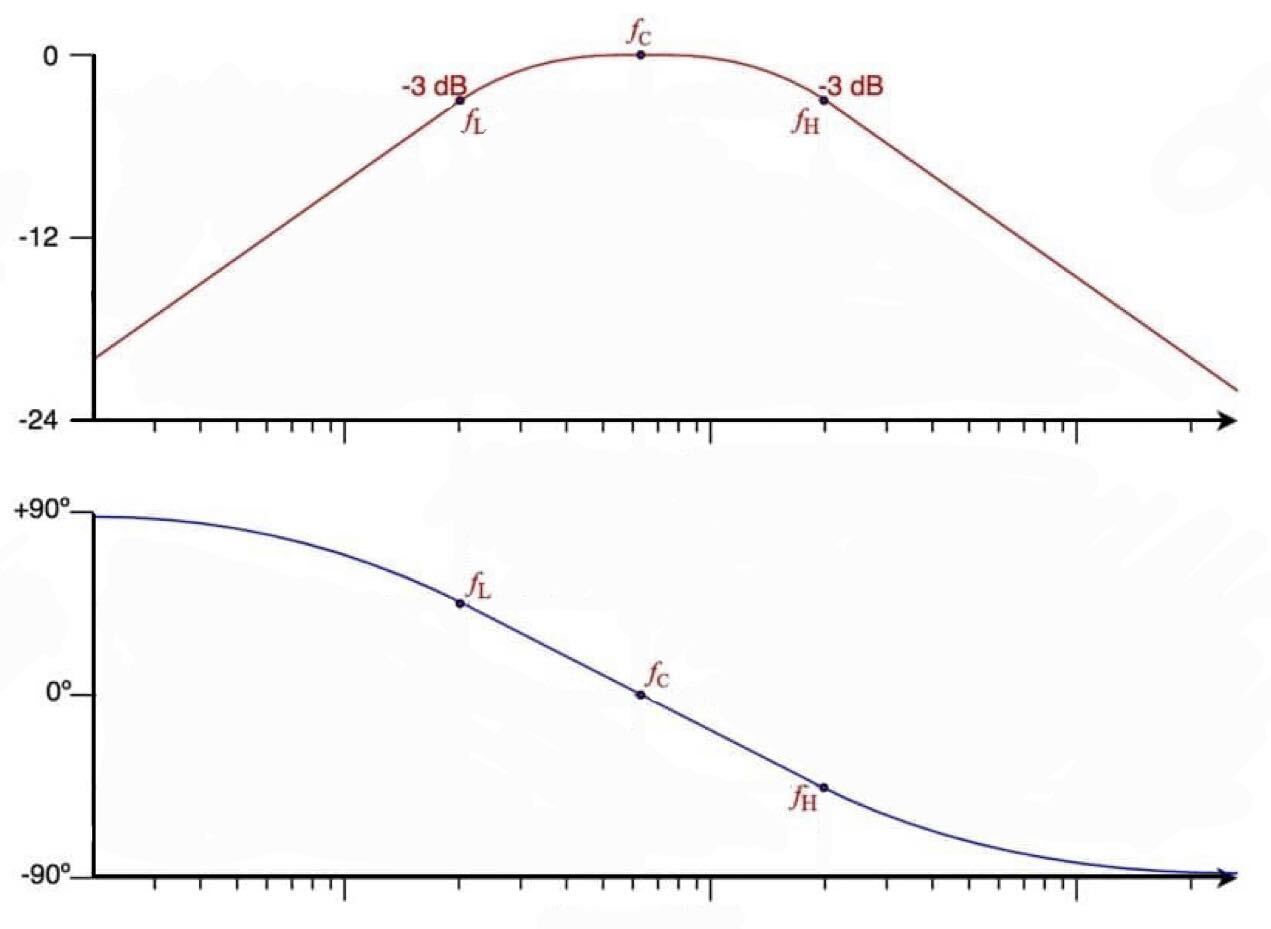
\includegraphics[scale=0.4]{D1/Images/response.jpg}
  \caption{Amplitude- og faserespons til et båndpass-filter.}
  \label{fig:4}
\end{figure}

Figur \ref{fig:4} viser eksempelvis et systems amplitude- og faserespons med bestemt $f_c$, der $f_L$ og $f_H$ er definert som frekvensene systemet demper amplituden med $-3 dB$.

Det finnes flere måter å designe kretser med båndpass-filter som funksjon. Et eksempel på en slik krets, som vil bli brukt i realiseringen er vist i figur \ref{fig:5}.

\begin{figure}[H]
  \centering
  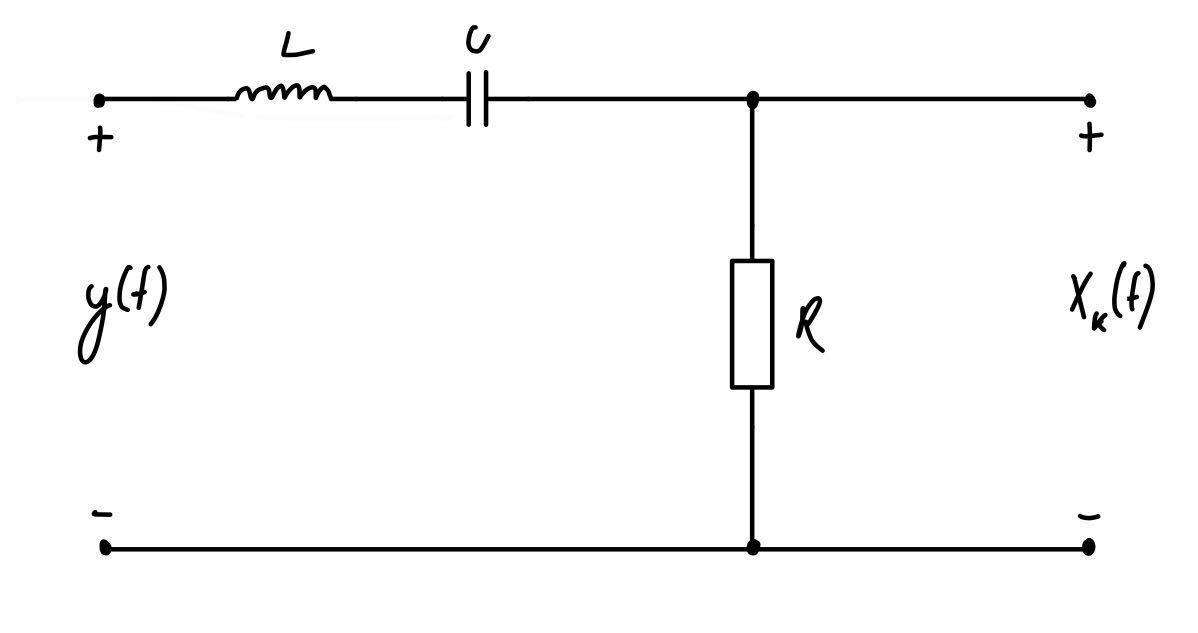
\includegraphics[scale=0.4]{D1/Images/bandpass.jpg}
  \caption{Båndstopp-filter med en resistor, kondensator og spole.}
  \label{fig:5}
\end{figure}

Båndbredden til bandpass-filteret defineres ut i fra avstanden mellom $f_L$ og $f_H$. For å oppnå så smal båndbredde som mulig kan man se på Q-faktoren til filteret ~\cite[Kva er eit “smalt” bandpassfilter?, s. 2)]{notat}

\begin{equation*}
    Q = \frac{f_0}{f_H-f_L} = \sqrt{\frac{L}{CR^2}}.
\end{equation*}

Stor Q-faktor betyr smalt filter, der spesielt resistorverdien blir viktig da den er kvadrert. Resistorverdien burde derfor være så lav som mulig for å oppnå en høyere Q-faktor, men ikke så lav at systemet ikke klarer å forsyne nok strøm.

Fra Designprosjekt 2 ~\cite[Prinsipiell løsning, s. 4)]{D2} kan  båndpass-filterets komponentverider regnes ut med likningen
\begin{equation}
    \label{eq:senterfrekvens}
    f_C = \frac{1}{\sqrt{2\pi LC}}.
\end{equation}

\subsection{SDR}
\label{sub:sdr}
Signal-til-Distorsjonsforhold sier noe om hvor godt ønsket resultatet $x_k(t)$ er i forhold til realisert resultat $\hat{x}_k(t)$, som er summen av $x_k(t)$ og et distorsjonssingal $d(t)$. Ved bruk av Parsevals sats forklart i ~\cite[Eit kvalitetsmål, s. 3-4)]{notat} er SDR gitt ved et logaritmisk mål 
\begin{equation*}
    SDR[dB] = 10lg\frac{V^2_{x_{k}}}{V^2_{\hat{x}_{k}}-V^2_{x_{k}}} 
\end{equation*}
der $V^2_{\hat{x}_{k}}$ er effektveridene (RMS) til $\hat{x}_k(t)$ og $V^2_{x_{k}}$ er amplituden til frekvenskomponenten til $x_k(t)$. SDR $\xrightarrow{}$ $\infty$ når $V^2_{\hat{x}_{k}}$ $\xrightarrow{}$ $V^2_{x_{k}}$, dermed impliserer en høy SDR et godt resultat. 

\section{Realisering og test}
\label{sec:realisering}
\subsection{Realisering}
Signalet som skal testes gjennom realisert system er et sinussignal $x_1(t)$ med en frekvens på $2525$ Hz, der systemet skal skal gi ut et signal $x_k(t)$ med dobbel frekvens; $5050$ Hz.

Realisering av systemet er vist i figur \ref{fig:oppkobling} med skjematisk oppkobling vist i figur \ref{fig:schematic} og komponentverdier i tabell \ref{tab:komp}.

\begin{figure}[H]
  \centering
  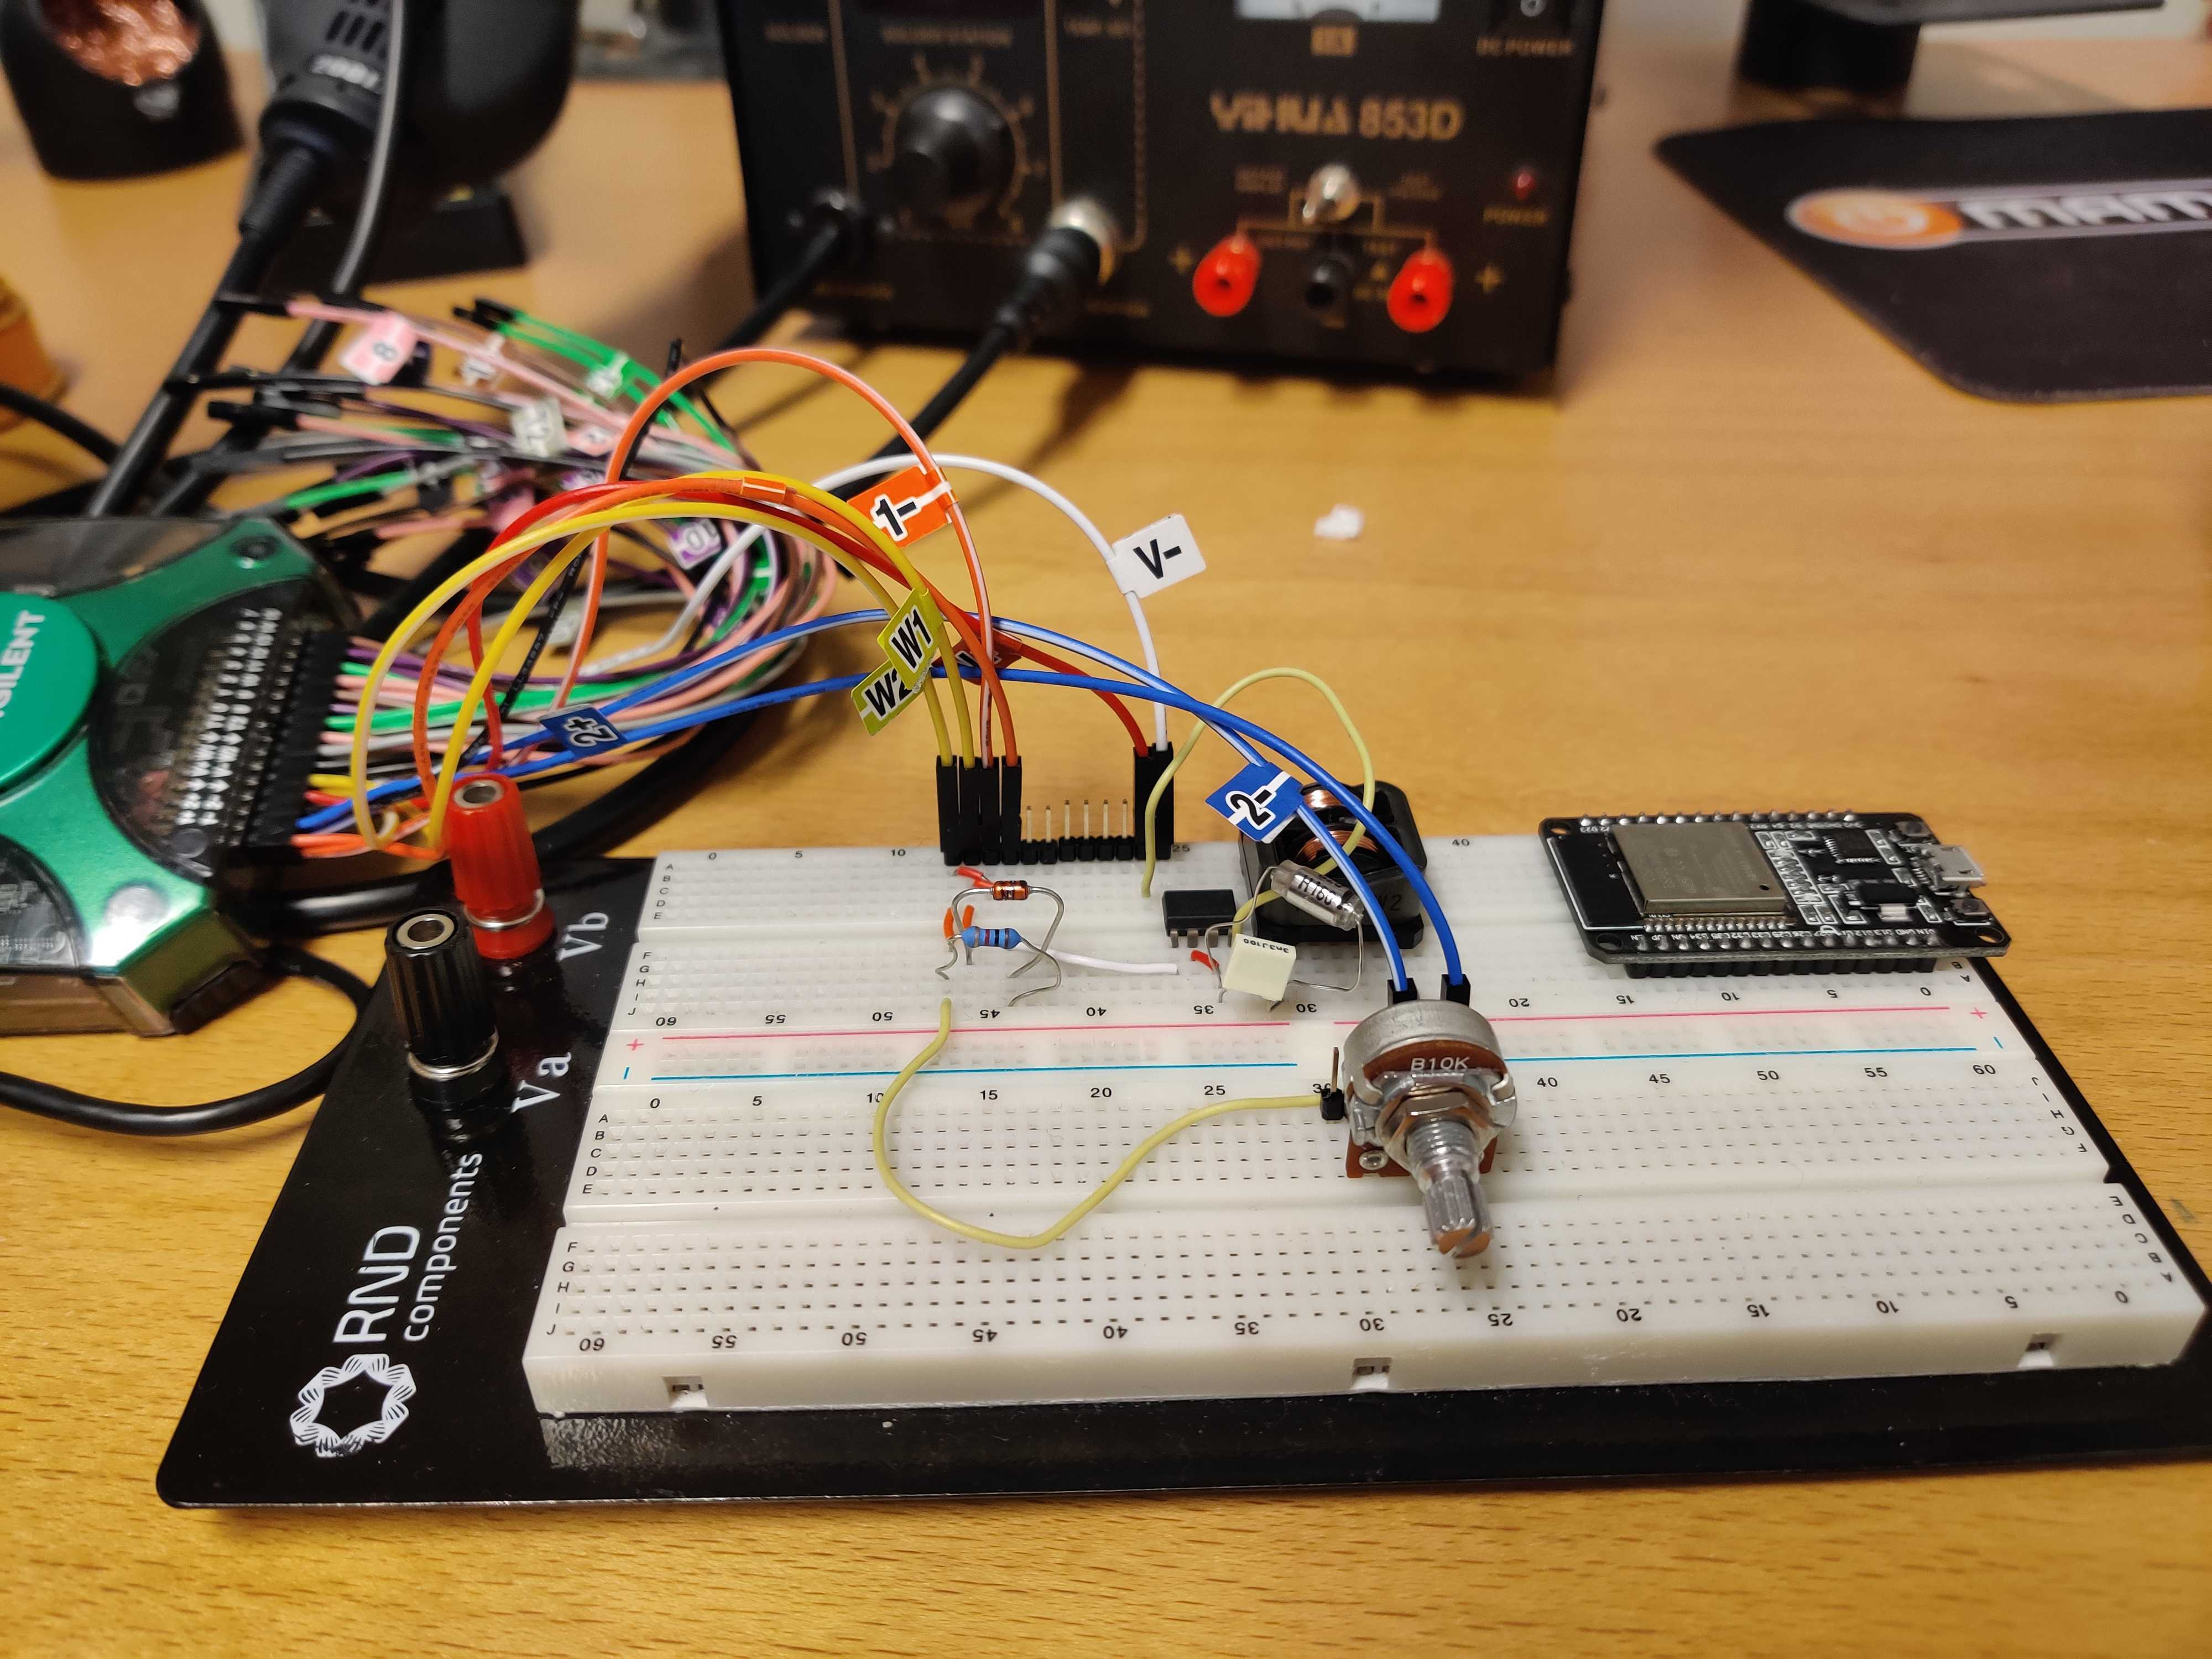
\includegraphics[scale=0.1]{D1/Images/circuit.jpg}
  \caption{Oppkobling av realisert krets på koblingsbrett.}
  \label{fig:oppkobling}
\end{figure}

\begin{figure}[H]
  \centering
  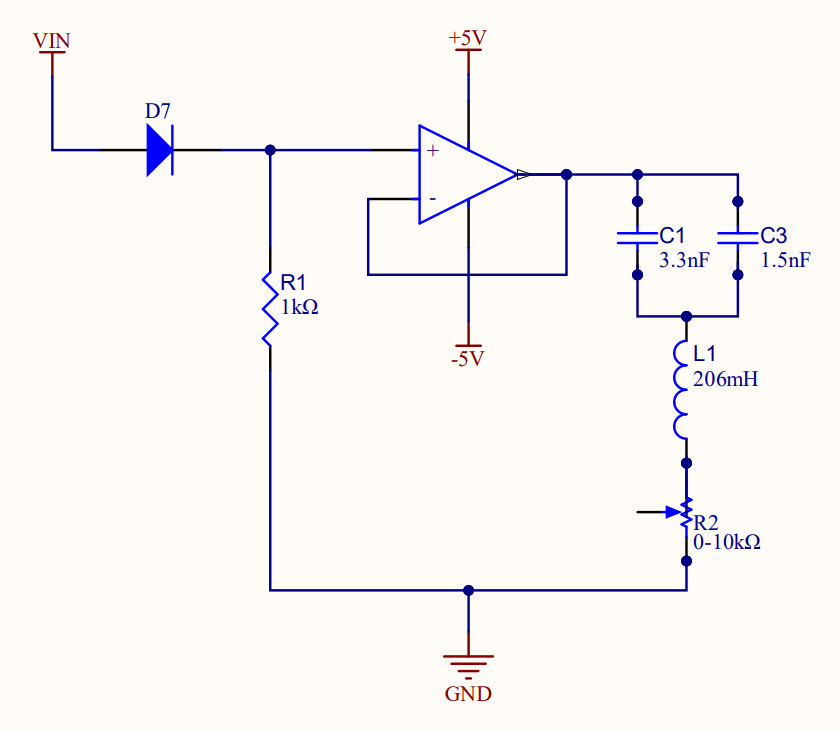
\includegraphics[scale=0.65]{D1/Images/altium.png}
  \caption{Skjematisk fremstilling av realisert krets.}
  \label{fig:schematic}
\end{figure}

\begin{table}[h]
  \centering
  \caption{Komponenter og deres standardverdier, samt målte verdier.}
  \label{tab:komp}
  \begin{tabular}{|c|c|c|}
    \hline\hline
    Komponenter & Standardverdi & Målt verdi \\
    \hline\hline
    $R_1$   & $1k$ $\Omega$ & $977$ $\Omega$\\
    \hline
    $R_2$   & $0-10k$ $\Omega$ & $230$ $\Omega$\\
    \hline
    $L_1$   & $100$ mH       & $206$ mH\\
    \hline
    $C_1$   & $3.3$ nF       & $3.32$ nF\\
    \hline
    $C_2$   & $1.5$ nF       & $1.50$ nF\\
    \hline
    $C_{total}$   & $4.8$ nF       & $4.82$ nF\\
    \hline\hline
    $D_1$          && \\
    \hline
    $LF353P$&&\\
    \hline
  \end{tabular}
\end{table}

Setter inn verdier for tilgjengelig spole $L$ til $206\mathrm{mH}$ og senterfrekvens $f_c$  og løser likning (\ref{eq:senterfrekvens}) for kondensatorverdien


\begin{equation*}
    C = \frac{1}{L(2\pi f_c)^2}
\end{equation*}
\begin{equation*}
    C = \frac{1}{206\mathrm{mH}(2\pi 5050\mathrm{Hz})^2} \approx 4.82 \mathrm{nF}
\end{equation*}



\subsection{Test}

Figur \ref{fig:osiloskop} plotter inngangsignalet $x_1(t)$ mot utgangssignalet $\hat{x}_k(t)$ der $\hat{x}_k(t)$ har en doblet frekvens med betydelig lavere amplitude enn ${x}_1(t)$. 

\begin{figure}[H]
  \centering
  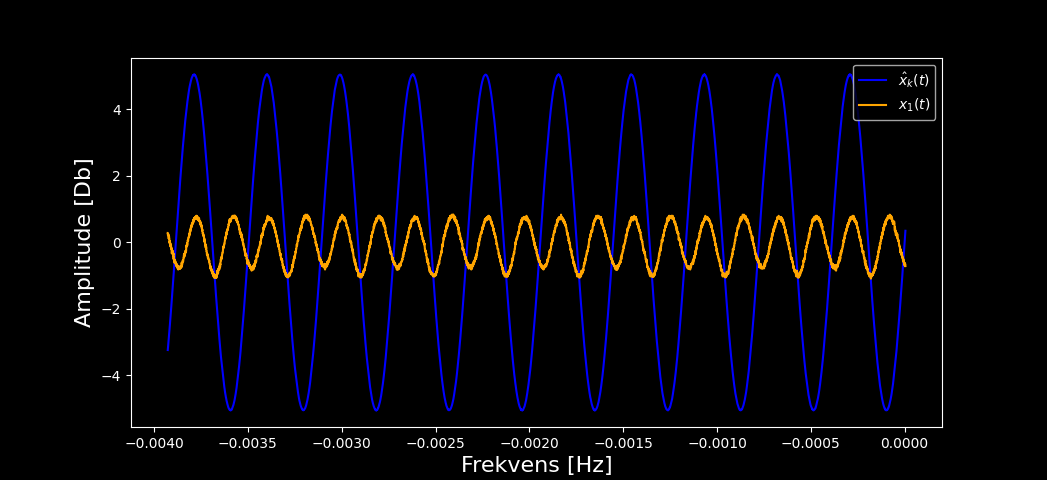
\includegraphics[scale=0.542]{D1/Images/Scope.png}
  \caption{Osiloskopanalyse av $\hat{x}_k(t)$ og $x_k(t)$ i programmet \emph{Waveforms}.}
  \label{fig:osiloskop}
\end{figure}
Ved hjelp av en spektrumanalysator er det mulig å identifisere frekvensene til utgangssignalet $\hat{x}_k(t)$ som vist i figur \ref{fig:spectrum}. Ønsket frekvens på $5050$ Hz har høyest amplitude, men det er flere harmoniske komponenter til stedet som skaper støy. 

\begin{figure}[H]
  \centering
  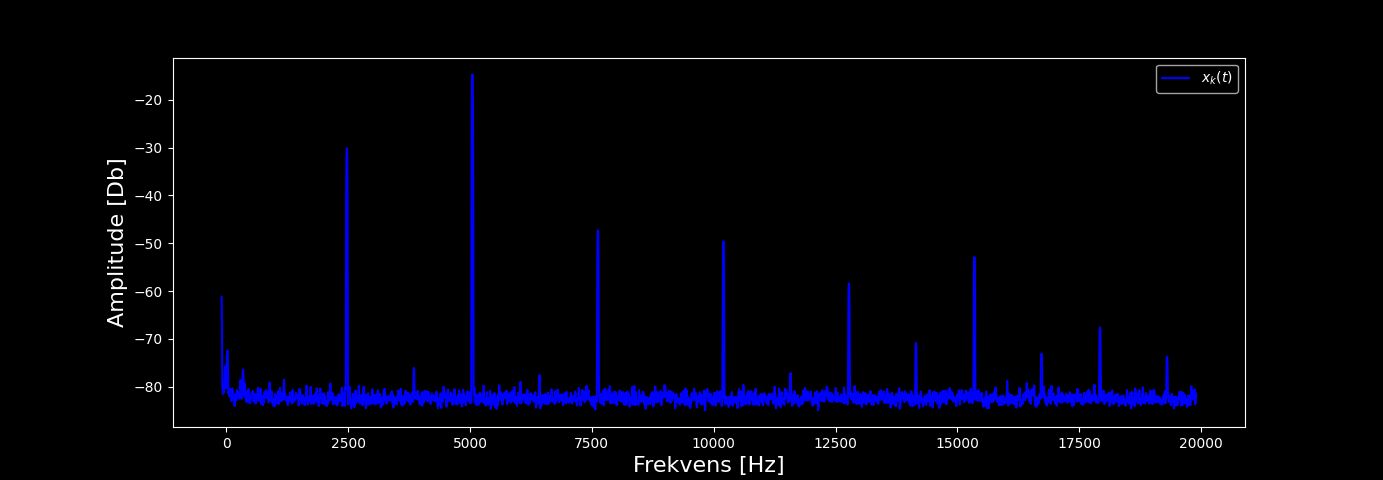
\includegraphics[scale=0.442]{D1/Images/Spectrum2.png}
  \caption{Spektrumanalyse av $\hat{x}_k(t)$ i programmet \emph{Waveforms}.}
  \label{fig:spectrum}
\end{figure}

For å analyserer utgangssignalet $\hat{x}_k(t)$ med SDR fra delkapittel \ref{sub:sdr} må verdier for $V^2_{\hat{x}_{k}}$ og $V^2_{x_{k}}$ anskaffes:

\begin{equation}
    SDR[dB] = 10lg\frac{V^2_{x_{k}}}{V^2_{\hat{x}_{k}}-V^2_{x_{k}}} .
    \label{eq:1}
\end{equation}

$V^2_{\hat{x}_{k}}$ kan måles av fra figur \ref{fig:spectrum2} til å være $\approx$ $197$ mV, og $V^2_{x_{k}}$ regnes ut fra osiloskopanalysen, vist i figur \ref{fig:osiloskop}, til å være $\approx$ $193.6$ mV.

Setter disse verdiene inn i (\ref{eq:1}) og får

\begin{equation*}
    SDR[dB] = 10lg\frac{(193.6mV)^2}{(193.2mV)^2-(193.6mV)^2} \approx 13.8
\end{equation*}

\begin{figure}[H]
  \centering
  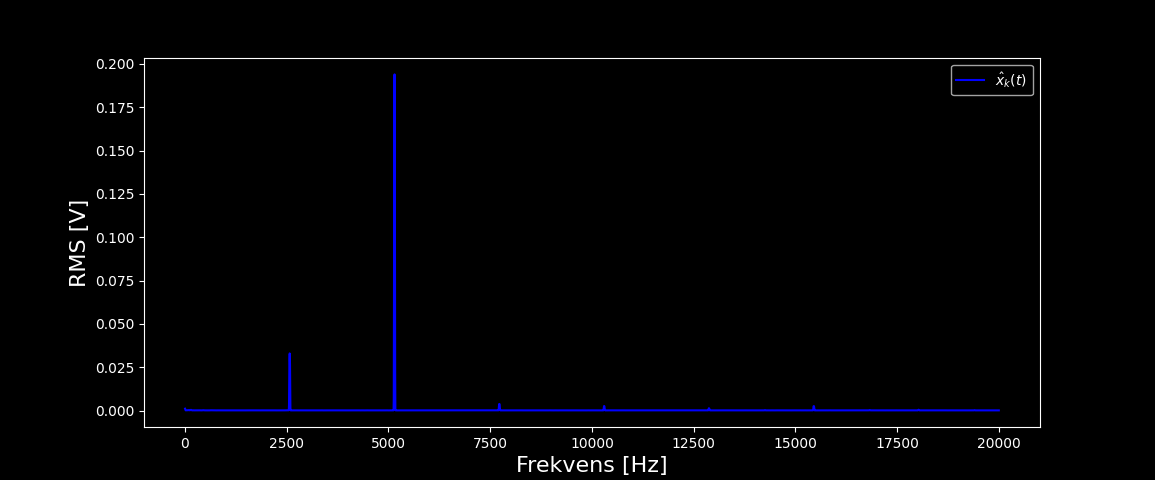
\includegraphics[scale=0.442]{D1/Images/Spectrum3.png}
  \caption{RMS-verdi til frekvenser av  $\hat{x}_{k}(t)$}.
  \label{fig:spectrum2}
\end{figure}


\section{Konklusjon}
\label{sec:konklusjon}

Systemet som ble beskrevet og implementert i dette notatet var en frekvensmultiplikator. Hensikten til dette systemet var å doble inngangssignalet, med minst mulig distorsjon på utgangssignalet. 
Etter testing og realisering ble et signal med dobbel frekvens oppnådd med en SDR målt til 13.8, med noe støy.

For å forbedre dette systemet kunne et smalere båndpassfilter blitt brukt, for å få mindre støy på utgangssignalet. Det kunne blitt realisert med flere filtre i serie eller en annen type med smalere båndbredde.

\section{Takk}

Takk til Orbit NTNU for å gi meg muligheten til bruk av lokalet og alt nødvendig utstyr, samt hjelp av flere medlemmer. 

Takker også mine medstudenter Mathias Askeland, Mahdan Gazimagamahev og Nikolai Andresen for hjelp til oppkobling, feilsøking og produktiv diskusjon rundt prosjektet.

\phantomsection
\addcontentsline{toc}{section}{Referanser}

\begin{thebibliography}{99}
    \bibitem{notat}
        Lundheim L., 
        \textit{Teknisk notat: Frekvensmultiplikator}, 
    	Elsys-2021-LL-1, 
    	NTNU,
    	2021.
    \bibitem{D2}
        Fløan F., 
        \textit{Designprosjekt 2: Støyfjerningsfilter}, 
    	NTNU,
    	2022.
\end{thebibliography}

\end{document}